% !TeX program = pdfLaTeX
\documentclass[12pt]{article}
\usepackage{amsmath}
\usepackage{graphicx,psfrag,epsf}
\usepackage{enumerate}
\usepackage{natbib}
\usepackage{textcomp}
\usepackage[hyphens]{url} % not crucial - just used below for the URL
\usepackage{hyperref}
\providecommand{\tightlist}{%
  \setlength{\itemsep}{0pt}\setlength{\parskip}{0pt}}

%\pdfminorversion=4
% NOTE: To produce blinded version, replace "0" with "1" below.
\newcommand{\blind}{0}

% DON'T change margins - should be 1 inch all around.
\addtolength{\oddsidemargin}{-.5in}%
\addtolength{\evensidemargin}{-.5in}%
\addtolength{\textwidth}{1in}%
\addtolength{\textheight}{1.3in}%
\addtolength{\topmargin}{-.8in}%

%% load any required packages here



% Pandoc citation processing

\usepackage{booktabs}
\usepackage{longtable}
\usepackage{array}
\usepackage{multirow}
\usepackage{wrapfig}
\usepackage{float}
\usepackage{colortbl}
\usepackage{pdflscape}
\usepackage{tabu}
\usepackage{threeparttable}
\usepackage{threeparttablex}
\usepackage[normalem]{ulem}
\usepackage{makecell}
\usepackage{xcolor}

\begin{document}


\def\spacingset#1{\renewcommand{\baselinestretch}%
{#1}\small\normalsize} \spacingset{1}


%%%%%%%%%%%%%%%%%%%%%%%%%%%%%%%%%%%%%%%%%%%%%%%%%%%%%%%%%%%%%%%%%%%%%%%%%%%%%%

\if0\blind
{
  \title{\bf An Examination of Sport Climbing Competition Format and
Scoring System}

  \author{
        Quang Nguyen \\
    \textit{Loyola University Chicago}\\
     and \\     Hannah Butler \\
    \textit{Colorado State University}\\
     and \\     Gregory J. Matthews \\
    \textit{Loyola University Chicago}\\
      }
  \maketitle
} \fi

\if1\blind
{
  \bigskip
  \bigskip
  \bigskip
  \begin{center}
    {\LARGE\bf An Examination of Sport Climbing Competition Format and
Scoring System}
  \end{center}
  \medskip
} \fi

\bigskip
\begin{abstract}
The purpose of this paper is to investigate the controversial
competition format and scoring system of sport climbing, which is one of
the sports making its debut on the Olympics stage at Tokyo 2020.
Climbing Olympians will participate in three disciplines (speed
climbing, bouldering, and lead climbing) for a single set of medals, and
a multiplied score of climbers' rankings in all three disciplines will
be used to determine the overall standings. This work finds great
evidence from historical data and simulations that speed climbing speed
climbing should be separated from the combined format and have its own
medals. Furthermore, it is shown that the product of ranks scoring
system violates the independence of irrelevant alternatives property.
\end{abstract}

\noindent%
{\it Keywords:} sport climbing, rankings, 2020 Summer Olympics
\vfill

\newpage
\spacingset{1.45} % DON'T change the spacing!

\hypertarget{introduction}{%
\section{Introduction}\label{introduction}}

In 2016, the International Olympic Committee (IOC) announced the
addition of five new sports to the 2020 Summer Olympics in Tokyo, Japan,
which would then reschedule for 2021 due to the impact of the COVID-19
global pandemic. The five new events added to Tokyo 2020's competition
program were baseball/softball, karate, skateboard, surfing, sports
climbing \citep{ioc2016}. One of the new sports, sport climbing, is
particularly interesting because of its scoring system which uses the
product of ranks across three disciplines to determine the medalists,
with the lowest rank product declared the winner.

\#While there are three main disciplines in sport climbing, the IOC only
allotted one set of medals per gender. So rather than choosing only a
single discipline, they chose to combine all three of the events
together to create a combined sport climbing event.

The three disciplines that comprise sport climbing at Tokyo 2020 are:
speed climbing, bouldering, and lead climbing. Speed climbing takes
place on a standardized course and competitors try to reach the top of
the course as fast as possible. For Tokyo 2020, speed climbing is being
contested in a head-to-head format with ranks determined by how far a
competitor advances in the bracket. In bouldering, contestants have a
fixed amount of time to complete as many courses as they can. Winners
are determined based on who completes the most courses and ties are
broken based on who had the fewest attempts. Ties are further broken by
the competitor achieved the most ``zone holds'', which are holds
approximately halfway through each course. Finally, in lead climbing, an
athlete gets one point for each hold that they reach, so whoever reaches
the highest point on the wall is the winner. Each lead climber only gets
one attempt and when they fall their attempt is over.

The decision to combine the three climbing events and only award one set
of medals for both men's and women's events in the Olympics has received
a large amount of criticism from climbing athletes all over the world
(CITATION NEEDED). In a series of interviews conducted by Climbing
Magazine in 2016, a number of climbers shared their thoughts and
concerns about the new Olympics climbing format. Climber Lynn Hill
compared the idea of combining speed climbing, bouldering, and lead
climbing to ``asking a middle distance runner to compete in the sprint''
(CITATION NEEDED). She then added ``Speed climbing is a sport within our
sport''. Other climbers also hold the same opinion as Hill regarding
speed climbing, using words and phrases like ``bogus'', ``a bummer'',
``less than ideal'', ``not in support'', and ``cheesy and unfair'' to
describe the new combined competition format. Courtney Woods stated
``Speed climbers will have the biggest disadvantage because their realm
isn't based on difficult movements''. Mike Doyle believed ``Honestly,
the people that will suffer the most are the ones that focus only on
speed climbing. Those skills/abilities don't transfer as well to the
other disciplines''. Most climbers also expressed their hope for a
change in the format in future tournaments, with some calling for each
discipline to have its own set of medals. See \citet{blanchard2016} for
more information on these interviews.

At the 2020 Summer Olympics, both sport climbing competitions for male
and female at the begin with 20 climbers who has previously qualified
for the Olympics from qualifying events held in 2019 and 2020. All 20
athletes compete in each of the three disciplines in the qualification
round, and their performances in each concentration are ranked from 1 to
20. A competitor's combined score is computed as the product of their
ranks in the three events; specifically, \begin{equation}
Score_i = R^S_i\times R^B_i\times R^L_i,
\end{equation} where \(R^S_i\), \(R^B_i\), and \(R^L_i\) are the ranks
of the \(i\)-th competitor in speed climbing, bouldering, and lead
climbing, respectively.

The 8 climbers with the lowest score (i.e.~lowest product of ranks
across the three disciplines) in the qualification round advance to the
finals where they once again compete in all three disciplines. The final
score for each person in the final stage is determined by multiplying
their ranks in each discipline, similar to the qualification round, with
the main difference being that there are only 8 competitors in the final
as opposed to 20 in the qualification round. The climbers with the
lowest, second lowest, and third lowest product of ranks in the final
wins the gold, silver, and bronze medal, respectively.

This type of scoring system heavily rewards high finishes and relatively
ignores poor finishes. For instance, if climber A finished 1st, 20th,
and 20th and climber B finished 10th, 10th, and 10th, climber B would
have a score of 1000 whereas climber A would have a much better score of
400, despite finishing last in 2 out of 3 of the events.

To the best of our knowledge, we know of no sporting event, team or
individual, that uses the product of ranks to determine an overall
rankings. There are examples of team sports that use the sum of ranks to
determine the winning team such as cross country, where the team with
the lowest sum of ranks of the top five runners is determined to be the
winner. For more detail on rank sum scoring, see \citet{hammond2007} and
\citet{boudreau2018}. In addition, some individual sports such as the
decathlon and heptathlon rely on a sum of scores from the ten or seven
events, however, these scores are not determined based on the ranks of
the competitors. That is, a decathlete's score is entirely based upon
their times, distances, and heights, and their overall score will be
exactly the same if the times, distances, and heights remain the same
regardless of the performance of other individuals. Full details of
decathlon scoring can be found in \citet{westera2006}.

The manuscript is outlined as follows. We first begin with some
descriptions of the data and methods in Section \ref{data-and-methods}.
Our analyses and results are then presented in Sections
\ref{simulations} and \ref{data-analysis}. Finally, in Section
\ref{conclusion-and-discussion}, we summarize up our main findings and
provide a discussion to close out the paper.

\hypertarget{data-and-methods}{%
\section{Data and Methods}\label{data-and-methods}}

Our first sets of data come from a simulation study that we conducted,
with the purpose of examining the rankings and scoring for climbers in
both qualification and final rounds. For each round, we performed 10000
simulations, and this was accomplished by randomly assigning the ranks
of each event to every participant, with the assumption that the ranks
are uniformly distributed. After the completion of the simulations, we
calculated the total scores for every simulated round, as well as the
final standings for the climbing athletes. The simulation results allow
to answer questions about various topics, including the distributions of
scores for qualifying and final rounds, and the probabilities of
advancing to the finals or winning a medal, given certain conditions.
First of all, Table 1 and Figure 1 are numerical and visual summaries of
climbing total score obtained from our simulated data for the
qualification and final rounds.

\begin{table}[H]

\caption{\label{tab:unnamed-chunk-4}Descriptive statistics of simulated scores for qualification and final rounds}
\centering
\begin{tabular}[t]{lrrrrrrrr}
\toprule
round & min & Q1 & median & Q3 & max & mean & sd & n\\
\midrule
Qualification & 1 & 240 & 684 & 1638 & 8000 & 1158.84378 & 1273.47884 & 200000\\
Final & 1 & 24 & 60 & 126 & 512 & 91.19935 & 91.11065 & 80000\\
\bottomrule
\end{tabular}
\end{table}

\begin{figure}

{\centering 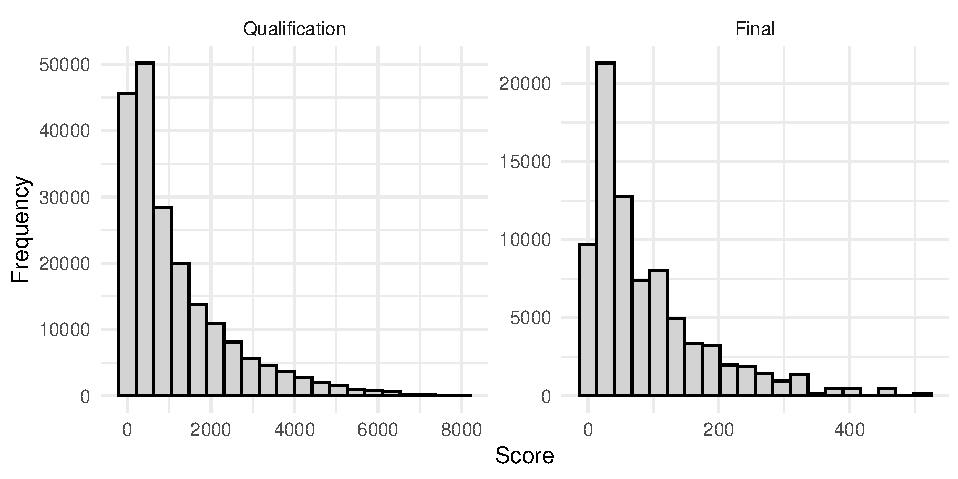
\includegraphics{draft_files/figure-latex/unnamed-chunk-5-1} 

}

\caption{Histogram of simulated scores for qualification and final rounds}\label{fig:unnamed-chunk-5}
\end{figure}

Additionally, we rely historical results from major climbing
competitions in recent years. We collected data on climbing contests
that took place between 2018 and 2020, where the combined format was
used to determine the scores and ranks of climbers. The events include
the 2020 Continental Championships of Europe, Africa, Oceania,
Pan-America; 2019 and 2018 World Championships; 2018 Asian Games; and
2018 Youth Olympics. Data were obtained from various sources, including
the event websites, Wikipedia, and the International Federation of Sport
Climbing (IFSC). The main attributes of our datasets are the name and
nationality of the climbers; bib number (for some competitions); the
finishing place of climbers in speed climbing, bouldering, and lead
climbing; the total score (which equals the product of event ranks); and
the final rank. We utilize this data to compute the correlations between
the event ranks and final table position, as well as to look at how
often the final orderings change if one athlete is dropped and the ranks
for each discipline are re-computed.

Paragraph on IIA/Social Choice

Suppose we have 3 people A, B, and C participating in a competition. If
A finishes in the first place and C is later disqualified and removed, A
should still win. If the original winner (A) loses the modified
competition (with C removed), then the Independence of Irrelevant
Alternatives has been violated.

Economics, psychology, probability theory. Connect with cross country in
previous section

First mentioned by Arrow (1951)
\url{https://cowles.yale.edu/sites/default/files/files/pub/mon/m12-all.pdf}

Luce (1959)
\url{http://www.scholarpedia.org/article/Luce\%27s_choice_axiom}

and Luce (1977)
\url{https://www.imbs.uci.edu/files/personnel/luce/pre1990/1977/Luce_JMP_1977a.pdf}

Ray (1973) \url{https://www.jstor.org/stable/1913820}

\hypertarget{simulations}{%
\section{Simulations}\label{simulations}}

\hypertarget{uniform-ranks}{%
\subsection{Uniform Ranks}\label{uniform-ranks}}

In this section, we discuss the results of our simulations described in
Section \ref{data-and-methods}. For the qualification round, our
simulation study shows that a climber is almost guaranteed to make the
final round if they win the first event or if they win at least one of
the three climbing concentrations (99.51\% and 99.48\% change of
advancing, respectively). On the other hand, finishing last in the first
event or in any event would certainly hurt an athlete's chance of
finishing in the top 8, as the probabilities of a climber advancing
given they finish last in the first and in any event are 0.1830 and
0.1885, respectively. In addition, the average score for qualification
positions 1 to 8 are displayed in Table 2. We notice that on average,
the minimum score that one should aim for in order to move on to the
final round is about 434 (for 8th rank).

\begin{table}[H]

\caption{\label{tab:unnamed-chunk-6}The average scores for the top 10 qualification ranks according to our simulations. A climber will secure a finalist spot if they finish in the top 8.}
\centering
\begin{tabular}[t]{rr}
\toprule
Rank & Average score\\
\midrule
1 & 36.0187\\
2 & 73.6111\\
3 & 115.3954\\
4 & 162.2263\\
5 & 216.0041\\
\addlinespace
6 & 278.1649\\
7 & 350.3272\\
8 & 434.5932\\
9 & 532.1383\\
10 & 642.3298\\
\bottomrule
\end{tabular}
\end{table}

Regarding the finals, a climber is very likely to finish in the top 3
and hence earn a medal if they win the first event (83.03\% chance) or
any event (85.01\% chance). Furthermore, according to our final
simulations, in order to obtain a climbing medal, the average scores
(rounded down) that put an athlete in position to receive gold, silver,
and bronze medals are 9, 20, and 33, respectively (see Table 3).

\begin{table}

\caption{\label{tab:unnamed-chunk-7}The average scores for all final ranks according to our simulations. Ranks 1, 2, and 3 are table positions that guarantee medalist status for climbers.}
\centering
\begin{tabular}[t]{rr}
\toprule
Rank & Average score\\
\midrule
1 & 9.6687\\
2 & 20.1844\\
3 & 33.3658\\
4 & 50.5734\\
5 & 75.2499\\
\addlinespace
6 & 110.7070\\
7 & 164.8258\\
8 & 265.0198\\
\bottomrule
\end{tabular}
\end{table}

\hypertarget{leave-one-climber-out}{%
\subsection{Leave-one-climber-out}\label{leave-one-climber-out}}

Another interesting question that we are interested in investigating is
``What would happen to the rankings if a single climber is removed?''.
This is related to the concept of independence of irrelevant
alternatives (IIA), as mentioned in Section \ref{data-and-methods}.

We would expect that if a climber with a high combined ranking is
removed from the list of competitors, the placement of lower-ranked
climbers will shift. In the most trivial case, if we were to remove the
3rd place climber, we would see 4th place climber shift to 3rd, 5th
place climber shift to 4th, etc. It is maybe less trivial that when a
climber is removed from the list, the placement of their higher-ranking
competitors may also shift. In other words, there is a non-zero
probability of seeing a change in the placement - particularly of
medalists - regardless of the fact that no changes occurred in the
performance of the remaining climbers. Real examples are given in
Section \ref{data-analysis}. In this section, we conduct simulations to
analyze the probability of seeing a reordering of medalists when one
non-medalist is removed from the list of finalists.

\hypertarget{data-analysis}{%
\section{Data Analysis}\label{data-analysis}}

\hypertarget{rank-correlation}{%
\subsection{Rank Correlation}\label{rank-correlation}}

For our analysis on the relationship between the rankings of the events
and the final result, we used data from the 2018 Youth Olympics Women's
Qualification. Figure 2 is a scatterplot and correlation matrix between
the ranks of the individual events and the final standings, with
Kendall's Tau \citep{kendall1938} as our measure of ordinal association
between the quantities. It is evidently clear that there exists a strong
and positive correlation between the ranks of bouldering and lead
climbing, and as a results, the standings of these two events are highly
correlated with the final rankings. On the other hand, the correlation
with the final rank is not as strong for speed climbing as the other two
events. Thus, speed climbers are facing a huge disadvantage in this
scoring system, compared to those that are specialized in the other two
concentrations. This validates the concerns of climbers in the interview
mentioned in Section \ref{introduction}. We also have evidence for these
correlations from the qualification rounds of the 2018 Asian Games
(Table 4), 2019 World Championship (Table 5), 2020 European Championship
(Table 6), and 2020 Pan-American Championships (Table 7).

\begin{figure}

{\centering 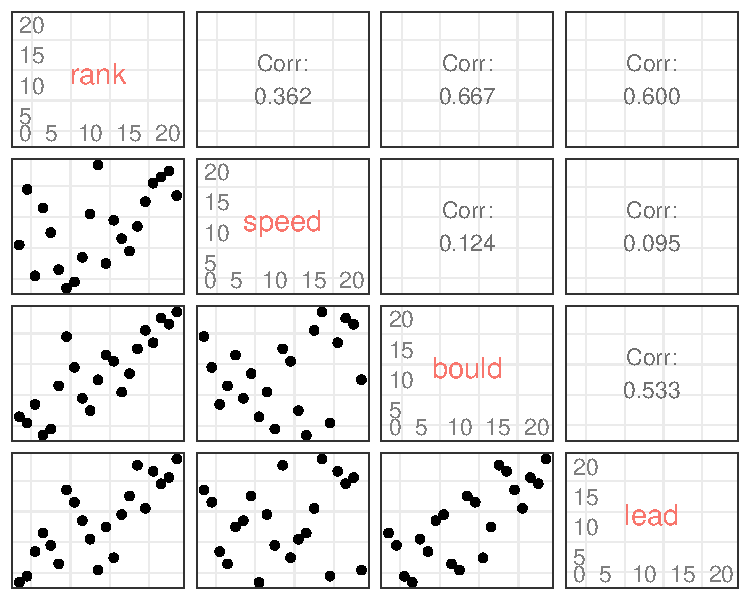
\includegraphics{draft_files/figure-latex/unnamed-chunk-9-1} 

}

\caption{Kendall's rank correlations - 2018 World Championship, Men's and Women's Qualifications}\label{fig:unnamed-chunk-9}
\end{figure}

\hypertarget{leave-one-climber-out-analysis}{%
\subsection{Leave-one-climber-out
Analysis}\label{leave-one-climber-out-analysis}}

Next, we perform analysis on the situations where a climber is dropped
from the original standings. We once again make use of data from the
2018 Youth Olympics for this analysis, but this time we examine the
final round of both men's and women's competitions.

Figure 3 shows the modified versions of the rankings after each ranked
climber is excluded for both gender events. We have clear evidence from
this plot that removing a single climber changes the rankings
drastically, especially order of medalists. One particular interesting
case is where an athlete's position change when someone who originally
finished behind them drops out. This situation is illustrated by panel 5
of the women's competition, where the fifth-place climber, Krasovskaia,
was excluded; and Meul, whose actual final rank was fourth, moved up to
the second spot and claim the silver medal.

Likewise, dropping a higher-ranked athlete could also result in a major
shake-up to the new orderings of players. This type of ranking change is
demonstrated by panel 1 and 2 of the men's facet. After dropping the
first ranked male contestant, Dohi; Schenk, who previously finished
fourth and outside of the medalist group now has the lowest score and
become the gold medal winner. A similar situation occurs in the case
where the second best competitor (Tanaka) was removed, which results in
a jump from fourth place to second place for Pan.

\begin{figure}

{\centering 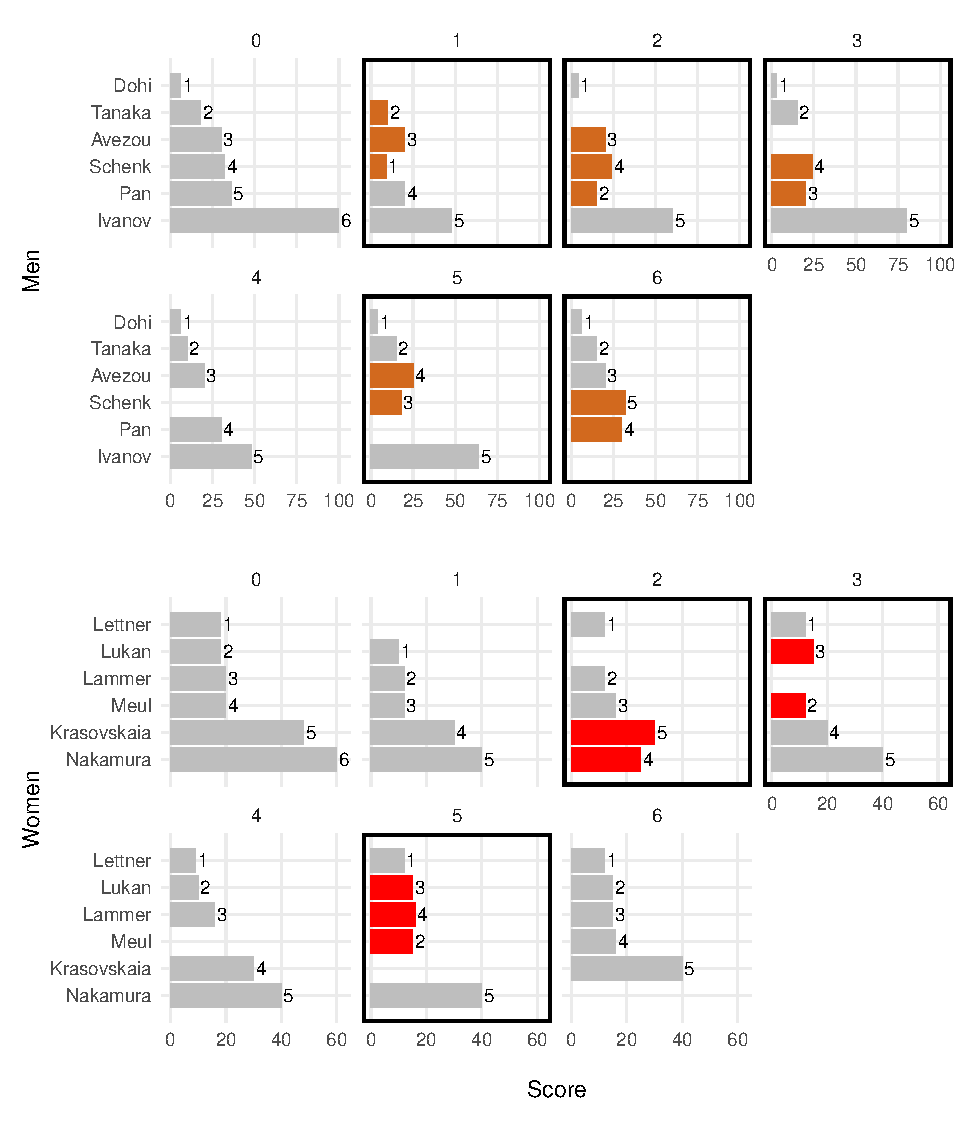
\includegraphics{draft_files/figure-latex/unnamed-chunk-12-1} 

}

\caption{This figure illustrates the changes to the final rankings of the 2018 Youth Olympics Men's and Women's Finals when we leave out one climber. For each gender competition, each panel represents the rank of the drop-out athlete, with 0 being the original final results. Each case with a change in rank orderings is highlighted by a black panel border, and any player with a rank change is represented by a red-filled bar}\label{fig:unnamed-chunk-12}
\end{figure}

\hypertarget{conclusion-and-discussion}{%
\section{Conclusion and Discussion}\label{conclusion-and-discussion}}

Overall

Speed climbers

There is a great dependence on irrelevant party.

Future work

Recommendations: climbers were right, need a change in format

\hypertarget{supplementary-material}{%
\section*{Supplementary Material}\label{supplementary-material}}
\addcontentsline{toc}{section}{Supplementary Material}

All of the materials related to this manuscript are publicly available
on GitHub at \newline \url{https://github.com/qntkhvn/climbing}.

\begin{table}[H]

\caption{\label{tab:unnamed-chunk-14}This table shows Kendall's rank correlation coefficients between the overall and individual discipline ranks for men's and women's sport climbing qualifications at the 2018 Asian Games}
\centering
\resizebox{\linewidth}{!}{
\begin{tabular}[t]{lrrrrrrrr}
\toprule
\multicolumn{1}{c}{} & \multicolumn{4}{c}{Men} & \multicolumn{4}{c}{Women} \\
\cmidrule(l{3pt}r{3pt}){2-5} \cmidrule(l{3pt}r{3pt}){6-9}
  & Overall & Speed & Bouldering & Lead & Overall & Speed & Bouldering & Lead\\
\midrule
Overall & 1.0000 & 0.5731 & 0.6760 & 0.6126 & 1.0000 & 0.5474 & 0.6878 & 0.7053\\
Speed & 0.5731 & 1.0000 & 0.3022 & 0.2174 & 0.5474 & 1.0000 & 0.2540 & 0.2947\\
Bouldering & 0.6760 & 0.3022 & 1.0000 & 0.6203 & 0.6878 & 0.2540 & 1.0000 & 0.6878\\
Lead & 0.6126 & 0.2174 & 0.6203 & 1.0000 & 0.7053 & 0.2947 & 0.6878 & 1.0000\\
\bottomrule
\end{tabular}}
\end{table}

\begin{table}[H]

\caption{\label{tab:unnamed-chunk-15}This table shows Kendall's rank correlation coefficients between the overall and individual discipline ranks for men's and women's sport climbing qualifications at the 2019 World Championships}
\centering
\resizebox{\linewidth}{!}{
\begin{tabular}[t]{lrrrrrrrr}
\toprule
\multicolumn{1}{c}{} & \multicolumn{4}{c}{Men} & \multicolumn{4}{c}{Women} \\
\cmidrule(l{3pt}r{3pt}){2-5} \cmidrule(l{3pt}r{3pt}){6-9}
  & Overall & Speed & Bouldering & Lead & Overall & Speed & Bouldering & Lead\\
\midrule
Overall & 1.0000 & 0.2632 & 0.3684 & 0.3474 & 1.0000 & 0.2316 & 0.5013 & 0.2526\\
Speed & 0.2632 & 1.0000 & -0.0947 & -0.3263 & 0.2316 & 1.0000 & 0.0686 & -0.4526\\
Bouldering & 0.3684 & -0.0947 & 1.0000 & 0.2000 & 0.5013 & 0.0686 & 1.0000 & 0.2902\\
Lead & 0.3474 & -0.3263 & 0.2000 & 1.0000 & 0.2526 & -0.4526 & 0.2902 & 1.0000\\
\bottomrule
\end{tabular}}
\end{table}

\begin{table}[H]

\caption{\label{tab:unnamed-chunk-16}This table shows Kendall's rank correlation coefficients between the overall and individual discipline ranks for men's and women's sport climbing qualifications at the 2020 European Championship}
\centering
\resizebox{\linewidth}{!}{
\begin{tabular}[t]{lrrrrrrrr}
\toprule
\multicolumn{1}{c}{} & \multicolumn{4}{c}{Men} & \multicolumn{4}{c}{Women} \\
\cmidrule(l{3pt}r{3pt}){2-5} \cmidrule(l{3pt}r{3pt}){6-9}
  & Overall & Speed & Bouldering & Lead & Overall & Speed & Bouldering & Lead\\
\midrule
Overall & 1.0000 & 0.0947 & 0.3810 & 0.2632 & 1.0000 & 0.1847 & 0.5358 & 0.5368\\
Speed & 0.0947 & 1.0000 & -0.1587 & -0.4316 & 0.1847 & 1.0000 & -0.1915 & -0.0897\\
Bouldering & 0.3810 & -0.1587 & 1.0000 & 0.2751 & 0.5358 & -0.1915 & 1.0000 & 0.5040\\
Lead & 0.2632 & -0.4316 & 0.2751 & 1.0000 & 0.5368 & -0.0897 & 0.5040 & 1.0000\\
\bottomrule
\end{tabular}}
\end{table}

\begin{table}[H]

\caption{\label{tab:unnamed-chunk-17}This table shows Kendall's rank correlation coefficients between the overall and individual discipline ranks for men's and women's sport climbing qualifications at the 2020 Pan American Championship}
\centering
\resizebox{\linewidth}{!}{
\begin{tabular}[t]{lrrrrrrrr}
\toprule
\multicolumn{1}{c}{} & \multicolumn{4}{c}{Men} & \multicolumn{4}{c}{Women} \\
\cmidrule(l{3pt}r{3pt}){2-5} \cmidrule(l{3pt}r{3pt}){6-9}
  & Overall & Speed & Bouldering & Lead & Overall & Speed & Bouldering & Lead\\
\midrule
Overall & 1.0000 & 0.5906 & 0.5556 & 0.6491 & 1.0000 & 0.5789 & 0.6140 & 0.5906\\
Speed & 0.5906 & 1.0000 & 0.2164 & 0.4035 & 0.5789 & 1.0000 & 0.2632 & 0.3099\\
Bouldering & 0.5556 & 0.2164 & 1.0000 & 0.2749 & 0.6140 & 0.2632 & 1.0000 & 0.3918\\
Lead & 0.6491 & 0.4035 & 0.2749 & 1.0000 & 0.5906 & 0.3099 & 0.3918 & 1.0000\\
\bottomrule
\end{tabular}}
\end{table}

\bibliographystyle{agsm}
\bibliography{references.bib}

\end{document}
